\documentclass[12pt,a4paper]{article}
\usepackage{amsmath,amssymb}
\usepackage{graphicx}
\usepackage{float}
\usepackage{tikz}
\usetikzlibrary{shapes, arrows, positioning}


\usepackage{amsmath,amssymb,mdframed}            % AMS package gives better equation layouts
\setcounter{page}{5}                    % sets first page number to 2
\setlength{\oddsidemargin}{-0.25in}     % set left margin
\setlength{\textwidth}{6.5in}           % set text width
\setlength{\topmargin}{-0.5in}          % controls layout at
\setlength{\headsep}{1cm}             % top of page
\setlength{\textheight}{9.0in}          % set text length



\makeatletter
\renewcommand{\@oddhead}{\hfill MA3600/14}  % sets header
\renewcommand{\@oddfoot}{\hfil \arabic{page} \hfil}    % sets page footer
\makeatother

\renewcommand{\labelenumi}{\arabic{enumi}} % Sets the first level of enumerate to be arabic (normal) numbers
\renewcommand{\labelenumii}{(\alph{enumii})} %Sets the second level of enumerate to be (a), (b), (c), .....
\renewcommand{\labelenumiii}{(\roman{enumiii})} % Sets the third level of enumerate to be (i), (ii), (iii), ....



\begin{document}
\begin{enumerate}
\setcounter{enumi}{3}

\renewcommand\labelenumi{\bfseries\theenumi.}

\item

    \begin{enumerate}
        \item Provide definitions for the following terms:
            \begin{itemize}
                \item Normal form game.  ~\hfill{[1]}

                \item Strictly dominated strategy.  ~\hfill{[1]}

                \item Weakly dominated strategy.  ~\hfill{[1]}

                \item Best response strategy.  ~\hfill{[1]}

                \item Nash equilibrium.  ~\hfill{[1]}
            \end{itemize}

        For the remainder of this question consider the battle of the sexes game:

            \[\begin{pmatrix}
            (3,2) & (0,0)\\
            (1,1) & (2,3)\\
            \end{pmatrix}\]

        \item By clearly stating the techniques used, obtain all (if any) pure Nash equilibria.

        ~\hfill{[4]}

        \item Plot the utilities to player 1 (the row player) assuming that the 2nd player (the column player) plays a mixed strategy: $\sigma_2 = (y,1-y)$.

        ~\hfill{[2]}

        \item Plot the utilities to player 2 (the column player) assuming that the 1st player (the row player) plays a mixed strategy: $\sigma_1 = (x,1-x)$.

        ~\hfill{[2]}

        \item Assuming that player 1 plays the mixed strategy $\sigma_1=(x,1-x)$, show that player 1's best response $x^*$ to a mixed strategy $\sigma_2 = (y,1-y)$ is given by:


            \[
            x^*=\begin{cases}
                0,&\text{ if } y < 1/2\\
                1,&\text{ if } y > 1/2\\
                \text{indifferent},&\text{ otherwise }\\
            \end{cases}
            \]

            Similarly show that player 2's best response $y^*$ is given by:

            \[
            y^*=\begin{cases}
                0,&\text{ if } x < 1/2\\
                1,&\text{ if } x > 1/2\\
                \text{indifferent},&\text{ otherwise }\\
            \end{cases}
            \]

        ~\hfill{[4]}

        \item Use the above to obtain all Nash equilibria for the game.

        ~\hfill{[2]}

        \item Confirm this result by stating, proving and using the Equality of Payoffs theorem.

        ~\hfill{[6]}

    \end{enumerate}

\newpage
\item

        Consider the following stage game:

        \[
        \begin{pmatrix}
        (2,2) & (5,0)\\
        (0,5) & (4,4)\\
        \end{pmatrix}
        \]

        This game shall be referred to as the Prisoner's Dilemma. The first strategy for both players will be referred to as `Cooperate' (\(C\)) and the second strategy will be referred to as `Defect' (\(D\)). \textbf{Players aim to minimise their payoffs.}

        Consider the following strategies:

            \begin{itemize}
                \item \(s_C\): Always cooperate;
                \item \(s_D\): Always defect;
                \item \(s_G\): Start by cooperating until your opponent defects at which point defect in all future stages.
            \end{itemize}

        Assume $S_1=S_2=\{s_C,s_D,s_G\}$.

    \begin{enumerate}

            \item Assuming a discounting factor of \(\delta\), obtain the utility to both players if the strategy pair \((s_C,s_C)\) is played.

            \hfill[2]

            \item Assuming a discounting factor of \(\delta\), obtain the utility to both players if the strategy pair \((s_D,s_D)\) is played.

            \hfill[2]

            \item For what values of \(\delta\) is \((s_G, s_G)\) a Nash equilibrium? \textbf{Recall that players aim to minimise their payoffs.}

            \hfill[5]

            \item Define the average payoff in an infinitely repeated game.

            \hfill[1]

            \item Plot the feasible average payoffs and the individually rational payoffs for the Prisoner's Dilemma. \textbf{Recall that players aim to minimise their payoffs.}

            \hfill[4]

            \item Prove the following theorem (\textbf{for games where players aim to minimise their payoffs}):

            ``Let \(u_1^*, u_2^*\) be a pair of Nash equilibrium payoffs for a stage game. For every individually rational pair \(v_1, v_2\) there exists \(\bar\delta\) such that for all \(1>\delta>\bar\delta>0\) there is a subgame perfect Nash equilibrium with payoffs \(v_1, v_2\).''

            \hfill[11]
    \end{enumerate}

\newpage
\item

    \begin{enumerate}
        \item Define a routing game \((G,r,c)\).

        \hfill{[2]}

        \item Define a Nash flow and using this definition obtain the Nash flow for the following game:

        \begin{center}
            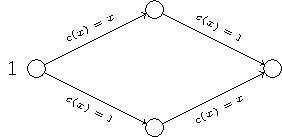
\includegraphics[width=.5\textwidth]{images/2013-2014-img01.pdf}
        \end{center}

        \hfill{[3]}

        \item Define an optimal flow and using this definition obtain the optimal flow for the above game.

        \hfill{[3]}

        \item State the theorem connecting the following function \(\Phi\) to the Nash flow of a routing game:

        \[\Phi(f)=\sum_{e\in E}\int_{0}^{f_e}c_e(x)dx\]

        \hfill{[2]}

        \item Using the theorem from (d) confirm the Nash flow previously found in (b).

        \hfill{[2]}

        \item State the theorem connecting the marginal cost \(c^*(x)=\frac{d(xc(x))}{dx}\) to the optimal flow of a routing game.

        \hfill{[2]}

        \item Using the theorem from (f) confirm the optimal flow previously found in (c) .

        \hfill{[2]}

        \item The expected time spent in an \(M/M/1\) queue at steady state is given by:

        $$W_q=\frac{\lambda}{\mu(\mu-\lambda)}$$

        where \(\mu,\lambda\) are the mean service and inter arrival rates and \(\lambda < \mu\) respectively. Explain how a system with two \(M/M/1\) queues and players choosing which queue to join can be studied using the following routing game:

        \begin{center}
            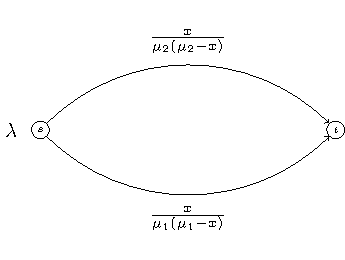
\includegraphics[width=.5\textwidth]{images/2013-2014-img02.pdf}
        \end{center}

        \hfill{[2]}

        \item Obtain the Nash and Optimal flows for the game in (h) with \(\mu_1=4,\mu_2=3\) and \(\lambda=2\).

        You might find it useful to know that the equation:

        \[x^4-2x^3+x^2-420x+324=0\]

        has a single solution in the range $0\leq x<2$ given by $x\approx 0.7715$.

        \hfill{[7]}

    \end{enumerate}
\end{enumerate}


\makeatletter
\renewcommand{\@oddfoot}{\hfil \arabic{page}X \hfil}    % sets last page footer
\makeatother

\end{document}
